% Compile with XeLaTeX or LuaLaTeX
\documentclass[12pt]{article}
\usepackage[margin=1in]{geometry}
\usepackage{graphicx}
\usepackage{microtype}
\usepackage[hidelinks]{hyperref}
\usepackage{xcolor}
\usepackage{ebgaramond} % Garamond-like body text
\usepackage{tikz}
\usetikzlibrary{positioning, arrows.meta}
\pagenumbering{gobble}

% ----- PDF metadata (helps when sharing the PDF) -----
\hypersetup{%
  pdftitle={Java Service on AWS EC2 via Infrastructure as Code},%
  pdfauthor={Akshat Sinha, Rakshika}%
}

% ----- Optional typography tweaks (leave commented if page count is tight) -----
% \linespread{1.03}

% ----- Optional: very subtle dark text (not recommended for academic submissions). Uncomment to enable. -----
% \AtBeginDocument{\color{black!98}}

% Subtle off-white background (1% yellow). For pure white, comment the next line.
\pagecolor{white!97.3!yellow}

\begin{document}
% ===== Title Page =====
\begin{titlepage}
\thispagestyle{empty}

\begin{minipage}[c][\textheight][s]{\textwidth}
\centering

{\itshape A}\\[6pt]
{\itshape Report Submitted}\\[6pt]
{\itshape for}\\[10pt]
{\Large\bfseries Project Review 1}\\[8pt]
{\itshape on the project entitled}\\[10pt]
{\LARGE\bfseries Java Service on AWS EC2 via Infrastructure as Code}\\[10pt]

{\itshape submitted as part of the requirements for the course}\\[6pt]
{\Large\bfseries BCSE408L - Cloud Computing (Theory Only)}\\[6pt]

\vspace{\stretch{1}}

{\Large\bfseries Bachelor of Technology}\\[6pt]
{\itshape in}\\[4pt]
{\Large\bfseries Computer Science \& Engineering}\\[10pt]

{\itshape by}\\[6pt]
{\large\bfseries Akshat Sinha (22BCE2218), Rakshika}\\[10pt]

{\itshape Under the guidance of}\\[6pt]
{\large\bfseries SIVA SHANMUGAM G}\\[12pt]

% Upload vit-logo.png into Overleaf (cannot link directly from the web)
\includegraphics[width=0.28\textwidth]{vit-logo.png}

\vspace{\stretch{1}}

{\large Department of Computer Science \& Engineering}\\
{\large Vellore Institute of Technology Vellore - 632014, INDIA}\\[8pt]
{\large 1 September 2025}

\end{minipage}
\end{titlepage}

\clearpage
\pagenumbering{arabic}\setcounter{page}{1}

% ===== Abstract =====
\section*{Abstract}
Using Amazon EC2, AWS CloudFormation, AWS Systems Manager, Amazon S3, Amazon CloudWatch, AWS CodeDeploy, and AWS Budgets, this work designs and operates a small Java Spring Boot REST service on AWS. The infrastructure is defined declaratively with CloudFormation, covering compute, identity and access, logging, and cost controls. The service runs on a t3.micro instance as a systemd unit; artifacts are stored in S3; IAM enforces least‑privilege access; Session Manager enables administrative access without public SSH; CloudWatch aggregates logs and alarms; Budgets provides spend guardrails; and CodeDeploy performs controlled in-place releases with automated health verification and rollback. The application exposes /health and /version endpoints and a minimal notes API used for functional and operational validation. We define three scenarios for evaluation: initial provisioning, version upgrade, and failure injection that triggers rollback and alerting. The result is a reproducible EC2‑based service that demonstrates core cloud practices—infrastructure as code, immutable artifacts, automated deployment, and basic observability—while keeping cost and complexity low.

\paragraph{Keywords:}
Amazon EC2; AWS CloudFormation; AWS Systems Manager; AWS CodeDeploy; Amazon S3; Amazon CloudWatch; Infrastructure as Code; DevOps; cost management.

\clearpage
\section{Introduction}
Cloud platforms make it possible to provision repeatable infrastructure and deliver updates safely. This report studies a minimal yet realistic pattern: a Java Spring Boot REST service on Amazon EC2 defined with AWS CloudFormation as Infrastructure as Code (IaC), operated with AWS Systems Manager, observed with Amazon CloudWatch, released with AWS CodeDeploy, and cost-guarded with AWS Budgets.

\subsection{Contributions}
\begin{itemize}
\item A minimal EC2-based architecture with declarative stacks for compute, identity, logging, and cost control.
\item Operational model using Session Manager (no public SSH), systemd-managed service, and CloudWatch alarms.
\item Controlled in-place releases with CodeDeploy and a failure scenario that triggers rollback and alerting.
\end{itemize}

\subsection{Scope and Assumptions}
\begin{itemize}
\item Single t3.micro instance in the default VPC; security group allows HTTP only.
\item Build artifacts in Amazon S3; logs and metrics in Amazon CloudWatch.
\item No NAT gateway or load balancer by default; a short demo workload with health checks.
\end{itemize}

\subsection{Paper Organization}
Section~\ref{sec:background} reviews background. Section~\ref{sec:architecture} details the system architecture. Section~\ref{sec:implementation} explains implementation. Section~\ref{sec:workflow} presents the deployment workflow and scenarios. Section~\ref{sec:evaluation} defines the evaluation plan and success criteria. Section~\ref{sec:plan} outlines the project plan and milestones. Section~\ref{sec:security} covers security considerations. Section~\ref{sec:limitations} outlines limitations and future work. Section~\ref{sec:conclusion} concludes.

\clearpage
\section{Background and Related Work}\label{sec:background}

Cloud computing offers elastic, metered resources delivered as services. In Infrastructure-as-a-Service (IaaS), Amazon EC2 provides virtual machines (instances) that boot from Amazon Machine Images and attach persistent EBS volumes. Network access is controlled by security groups. This project uses a small general-purpose instance class to keep cost low while showing standard operations for a production-style service.

Infrastructure as Code (IaC) captures the desired state of cloud resources in versioned templates. AWS CloudFormation builds and updates stacks from these templates, tracks dependencies, and supports change sets and drift detection. IaC improves repeatability, review, and rollback. Alternative tools such as Terraform and AWS CDK provide similar goals; we select CloudFormation for native integration and a smaller toolchain.

Application release strategies aim to reduce risk. In-place deployment replaces the application on existing hosts and is simple but has brief service impact if not orchestrated. Blue/green keeps two environments and shifts traffic between them, which reduces risk at the cost of extra capacity. Canary is a controlled form of blue/green that shifts a small percentage first, then the remainder after health verification. AWS CodeDeploy supports these patterns with lifecycle hooks and automatic rollback on failed health checks or alarms.

Operations require visibility and safe access. Amazon CloudWatch aggregates logs and metrics and can raise alarms on resource health and application errors. AWS Systems Manager Session Manager provides shell access without opening public SSH, and Run Command supports controlled changes. IAM enables least-privilege roles for instances and automation, reducing the blast radius of any fault.

Cost governance is essential even for small projects. AWS Budgets warns when actual or forecasted spend crosses a threshold. Tagging resources by project and environment helps with cost allocation and cleanup. Avoiding fixed-cost components (for example NAT gateways and always-on load balancers) keeps idle cost minimal while preserving the learning goals.

Related work includes serverless designs that replace EC2 with AWS Lambda and API Gateway, and alternative IaC and deployment stacks (Terraform, CDK, GitHub Actions). We retain EC2 to demonstrate virtualization concepts, system initialization with systemd, and host-level observability while still applying modern automation practices.

\begin{table}[h]
\centering
\caption{Release strategies used in practice}
\begin{tabular}{p{0.22\textwidth}p{0.68\textwidth}}
\hline
In-place & Replace the application on current hosts; lowest cost; brief risk window if not drained. \\
Blue/green & Maintain two environments and switch traffic; safer rollbacks; requires extra capacity. \\
Canary & Shift a small percentage first, then the rest after health checks; balances safety and speed. \\
\hline
\end{tabular}
\end{table}

\clearpage
\section{System Architecture}\label{sec:architecture}

\subsection{Overview}
The system hosts a small Java Spring Boot REST service on a single Amazon EC2 instance and augments it with declarative infrastructure, safe access, logging, and cost control. Core services are: Amazon EC2 (compute), AWS CloudFormation (IaC), AWS Identity and Access Management (IAM), AWS Systems Manager Session Manager (administrative access), Amazon S3 (artifact storage), Amazon CloudWatch (logs and alarms), AWS CodeDeploy (in-place releases with rollback), and AWS Budgets (spend guardrail). The instance runs in the default VPC with a security group that permits inbound HTTP and denies public SSH.

\subsection{Component responsibilities}
\begin{itemize}
\item EC2 instance: Amazon Linux 2023 t3.micro; EBS root volume; systemd unit launches the Spring Boot jar; Instance Metadata Service v2 enabled.
\item IAM instance profile: least‑privilege permissions for S3 object read, CloudWatch logs, and SSM core.
\item CloudFormation stack: declares S3 bucket, IAM roles and policies, security group, EC2 instance, CloudWatch log group and alarms, and a budget.
\item Systems Manager: Session Manager for shell access without open SSH; Run Command for controlled operational steps.
\item S3 artifact bucket: versioned object storage for application zips and configuration assets.
\item CloudWatch: application and system logs, CPU/StatusCheck alarms, optional custom metrics from the app.
\item CodeDeploy (optional in minimal run): coordinates in-place deployments using lifecycle hooks and health verification.
\item Budgets: notifies on actual or forecasted spend crossing a threshold.
\end{itemize}

\subsection{Networking and access}
The instance resides in a public subnet of the default VPC and receives a public IPv4 address. Inbound access is restricted to TCP/80; SSH is closed. Administrative sessions use Session Manager (encrypted channels, audit logs in CloudWatch or S3 if enabled). Outbound egress is open to AWS endpoints needed by S3, CloudWatch, and Systems Manager.

\subsection{Deployment model}
Build artifacts are produced as a fat jar, packaged with auxiliary scripts, and stored in S3. Releases are executed either via CodeDeploy (recommended for clean versioning and rollback) or via Systems Manager Run Command (lightweight). Health is checked via the /health endpoint; failures during installation or validation trigger rollback when using CodeDeploy.

\subsection{Configuration and secrets}
Application parameters (for example, port, log level, feature flags) are externalized. Non‑sensitive values are set as environment variables; sensitive values should use SSM Parameter Store with KMS encryption. The instance role grants read access only to the required parameter paths.

\subsection{Reliability, observability, and cost}
Systemd restarts the service on failure. CloudWatch captures instance and application logs and raises alarms on StatusCheckFailed and sustained CPU pressure. The budget is set low (e.g., \$5/month) and can be tuned per environment. All resources carry project and owner tags to simplify accounting and teardown.

% Optional diagram: add to preamble \usepackage{tikz} and \usetikzlibrary{positioning,arrows.meta}
\begin{figure}[t]
\centering
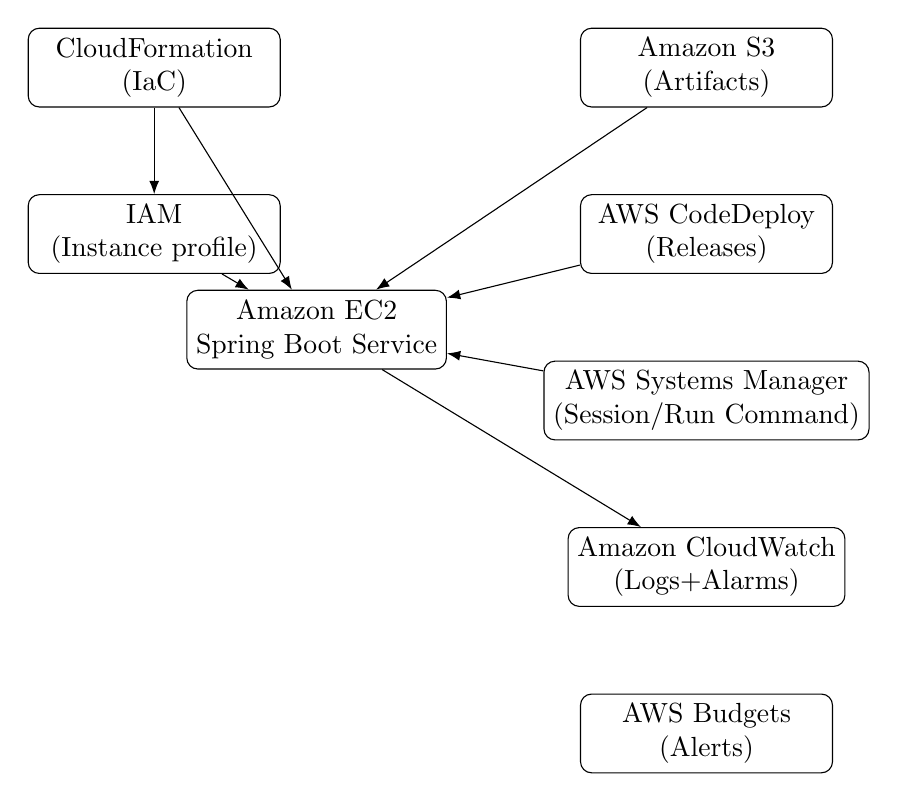
\begin{tikzpicture}[node distance=1.1cm and 1.6cm,>=Latex]
\tikzset{box/.style={draw,rounded corners,align=center,minimum width=3.2cm,minimum height=1.0cm}}
\node[box] (cfn) {CloudFormation\\(IaC)};
\node[box,below=of cfn] (iam) {IAM\\(Instance profile)};
\node[box,right=3.8cm of cfn] (s3) {Amazon S3\\(Artifacts)};
\node[box,below=of s3] (cd) {AWS CodeDeploy\\(Releases)};
\node[box,below=of cd] (ssm) {AWS Systems Manager\\(Session/Run Command)};
\node[box,below=of ssm] (cw) {Amazon CloudWatch\\(Logs+Alarms)};
\node[box,below=of cw] (bud) {AWS Budgets\\(Alerts)};

\node[box,below right=0.2cm and -1.2cm of iam] (ec2) {Amazon EC2\\Spring Boot Service};

\draw[->] (cfn) -- (ec2);
\draw[->] (iam) -- (ec2);
\draw[->] (s3) -- (ec2);
\draw[->] (cd) -- (ec2);
\draw[->] (ssm) -- (ec2);
\draw[<-] (cw) -- (ec2);
\draw[->] (cfn) -- (iam);
\end{tikzpicture}
\caption{Logical architecture and service responsibilities.}
\label{fig:architecture}
\end{figure}

\clearpage
\section{Implementation and Methods}\label{sec:implementation}

\subsection{Infrastructure-as-Code templates}
A single CloudFormation stack declares all required resources: an Amazon S3 bucket for artifacts, an IAM role and instance profile with least-privilege policies (S3 object read, CloudWatch logs, SSM core), a security group that allows inbound TCP/80 only, a t3.micro Amazon EC2 instance with an EBS root volume, a CloudWatch log group and two alarms (StatusCheckFailed and sustained CPU), and an AWS Budget. Parameters expose instance type, artifact bucket name, budget amount, and application port; tags record project, owner, and environment. Change sets are used for safe updates and to detect drift.

\subsection{Instance bootstrapping and runtime}
The instance runs Amazon Linux 2023 and Amazon Corretto 17. Cloud-init user data performs: package updates; creation of a dedicated \texttt{app} user; installation and configuration of the CloudWatch agent; creation of \texttt{/opt/app} and \texttt{/var/log/app}; and installation of a systemd unit that runs the Spring Boot fat jar with restart-on-failure policy. Instance Metadata Service v2 is enforced. On first boot, if an artifact is present in S3 it is downloaded and started; otherwise a placeholder service responds at \texttt{/health}.

\subsection{Application}
The service is a minimal REST endpoint set used for operational validation: \texttt{/health} (readiness probe), \texttt{/version} (build metadata), and a small notes API with create/read/update/delete to exercise logs and updates. Configuration (port, log level, feature flags) is externalized via environment variables; sensitive values, if any, are placed in SSM Parameter Store under a project-specific path with KMS encryption and read-only access from the instance role.

\subsection{Release and rollback}
Releases are executed with AWS CodeDeploy in in-place mode. The artifact is a zip containing the fat jar, an \texttt{appspec.yml}, and lightweight lifecycle scripts. The hooks perform: \emph{BeforeInstall} (stop service), \emph{AfterInstall} (unpack files, set ownership), \emph{ApplicationStart} (enable and start the systemd unit), and \emph{ValidateService} (HTTP check on \texttt{/health}). Auto-rollback is enabled on deployment failure or alarm breach; the previous artifact is restored and the service is restarted. For very small demos, Systems Manager Run Command can replace CodeDeploy with a shorter path at the cost of automated rollback.

\subsection{Observability and cost controls}
System logs and application logs are routed to an application-specific CloudWatch log group. Alarms fire on instance status failure and on sustained CPU utilization, notifying the default SNS topic or email (course policy dependent). The budget is set low (e.g., \$5/month) with forecasted and actual alerts. All resources are tagged to support allocation and cleanup.

\subsection{Verification}
Provisioning is successful when the stack completes without error and the instance serves \texttt{/health} with HTTP~200. A release is considered successful when CodeDeploy reports \emph{Succeeded} and the \texttt{/version} endpoint reflects the new build. A negative test intentionally fails \emph{ValidateService} to confirm automatic rollback and alarms.

\section{Deployment Workflow and Scenarios}\label{sec:workflow}

\subsection{Workflow}
\begin{enumerate}
\item Build: package the Spring Boot service as a fat jar; embed build time and git commit for \texttt{/version}.
\item Package: zip the jar with \texttt{appspec.yml} and small lifecycle scripts.
\item Publish: upload the artifact to Amazon S3 under a versioned key (e.g., \texttt{java-service/\{commit\}.zip}); retain at least one prior version.
\item Provision/Update: apply the CloudFormation stack; confirm stack events show \emph{UPDATE\_COMPLETE}.
\item Deploy: create a CodeDeploy in-place deployment targeting the EC2 instance (tagged \texttt{App=JavaService}).
\item Validate: lifecycle hook requests \texttt{GET /health}; deployment succeeds only on HTTP 200; logs stream to CloudWatch.
\item Rollback policy: enable automatic rollback on deployment failure or alarm breach; CodeDeploy restores the last good artifact.
\item Teardown (optional): delete the stack and empty the artifact bucket after the review to control cost.
\end{enumerate}

\subsection{Scenarios}
\paragraph{S1: Initial provisioning and v1 release}
Create the stack, publish \texttt{v1}, and deploy. Success criteria: stack completes; instance reachable on HTTP 80; \texttt{/health} returns 200; \texttt{/version} shows the expected commit.

\paragraph{S2: Version upgrade (v1 $\rightarrow$ v2)}
Change a visible response (e.g., banner text or minor endpoint behavior), publish \texttt{v2}, and redeploy. Success criteria: CodeDeploy status \emph{Succeeded}; \texttt{/version} reflects the new commit; no alarms fire.

\paragraph{S3: Failure injection and rollback}
Introduce a deliberate failure (e.g., make \texttt{/health} return 500 during \emph{ValidateService}) and deploy. Expected outcome: CodeDeploy marks \emph{Failed}, performs automatic rollback to the previous artifact, and service recovers without manual intervention.

\subsection{Measurements and evidence}
\begin{itemize}
\item Deploy duration: CodeDeploy timeline from \emph{Created} to \emph{Succeeded/Failed}.
\item Health outcomes: HTTP status for \texttt{/health} before and after each deployment.
\item Resource signals: CPU and StatusCheck alarms in CloudWatch (should remain normal for S1--S2; S3 triggers failure then recovery).
\item Cost: monthly budget threshold and a short snapshot of estimated spend during the review window.
\end{itemize}

\section{Evaluation Plan and Success Criteria}\label{sec:evaluation}

\subsection{Objectives}
Validate that (i) infrastructure provisions repeatably, (ii) the service updates safely with rollback, (iii) logging and alarms provide actionable signals, and (iv) monthly cost stays low.

\subsection{Metrics and targets}
\begin{table}[h]
\centering
\caption{Planned evaluation metrics}
\begin{tabular}{p{0.33\textwidth}p{0.58\textwidth}}
\hline
Metric & Target \\
\hline
Provision success & 100\% stack completion without manual fixes. \\
Deployment success & 100\% for normal updates (S2). \\
Rollback effectiveness & Service restored to last good version after induced failure (S3). \\
Deployment time & $\leq$5 minutes per release (build excluded). \\
Health during update & $\geq$99\% /health success over the update window. \\
Cost guardrail & Forecasted monthly spend $\leq$\$5 with alerting enabled. \\
\hline
\end{tabular}
\end{table}

\subsection{Planned scenarios}
S1: initial provisioning and v1 release; S2: v1$\rightarrow$v2 update; S3: induced failure triggering rollback. Evidence will be collected from CloudFormation events, CodeDeploy deployment details, and CloudWatch logs/alarms; results will be summarized at the final review.

\section{Project Plan and Milestones}\label{sec:plan}

\begin{itemize}
\item M0: Design and Project Review 1 submission
\item M1: CloudFormation stack (EC2, IAM, SG, S3, logs, budget)
\item M2: Instance bootstrap (systemd, SSM, logging)
\item M3: Artifact packaging and first deploy (v1)
\item M4: Alarms and budget verification
\item M5: Update (v2) and rollback scenario (S3)
\item M6: Final write-up and demo
\end{itemize}

\subsection{Risks and mitigations}
Quota or permission errors (pre-check IAM and quotas); cost creep (budget alerts, avoid fixed-cost components); time constraints (small milestones and teardown after tests).

\section{Security Considerations}\label{sec:security}
\begin{itemize}
\item Least privilege: the instance profile grants only S3 object read, CloudWatch logs, and SSM core; resource paths are scoped by prefix and tag conditions.
\item Network: security group allows inbound TCP/80 only; SSH closed; egress limited to required AWS endpoints where feasible.
\item Access: administrative sessions use Systems Manager Session Manager; actions are audited (CloudWatch/CloudTrail if enabled).
\item Host hardening: IMDSv2 enforced; systemd restarts on failure; regular OS updates (via SSM Patch Manager in later milestone).
\item Secrets/config: non‑sensitive via environment variables; sensitive values planned in SSM Parameter Store with KMS encryption and read‑only access.
\item Artifact integrity: S3 versioning retained; optional checksum verification or code‑signing planned for later milestone.
\end{itemize}

\section{Limitations and Future Work}\label{sec:limitations}
\begin{itemize}
\item Single instance in default VPC; no multi‑AZ or auto scaling.
\item No load balancer by default; blue/green or canary may be demonstrated later with a short‑lived ALB.
\item No database layer; current API is for operational validation only.
\item Manual approvals and richer CI/CD, code‑signing, and parameterized environments (dev/stage) are planned for the final review.
\end{itemize}

\section{Conclusion}\label{sec:conclusion}
This review defined a minimal, cloud‑oriented architecture for a Java Spring Boot service on Amazon EC2 using Infrastructure as Code. The design emphasizes repeatable provisioning, safe operational access without public SSH, and basic observability and cost control. The next milestone implements the stack, performs the first release, and prepares the update and rollback scenarios for evaluation.

\section*{References}
\begin{thebibliography}{9}

\bibitem{ec2}
Amazon Web Services, ``Amazon EC2 User Guide for Linux Instances,'' Available at: \url{https://docs.aws.amazon.com/AWSEC2/latest/UserGuide/}. Accessed: 1 Sept. 2025.

\bibitem{cfn}
Amazon Web Services, ``AWS CloudFormation User Guide,'' Available at: \url{https://docs.aws.amazon.com/AWSCloudFormation/latest/UserGuide/}. Accessed: 1 Sept. 2025.

\bibitem{codedeploy}
Amazon Web Services, ``AWS CodeDeploy User Guide,'' Available at: \url{https://docs.aws.amazon.com/codedeploy/latest/userguide/}. Accessed: 1 Sept. 2025.

\bibitem{ssm}
Amazon Web Services, ``AWS Systems Manager User Guide,'' Available at: \url{https://docs.aws.amazon.com/systems-manager/latest/userguide/}. Accessed: 1 Sept. 2025.

\bibitem{cloudwatch}
Amazon Web Services, ``Amazon CloudWatch User Guide,'' Available at: \url{https://docs.aws.amazon.com/AmazonCloudWatch/latest/monitoring/}. Accessed: 1 Sept. 2025.

\bibitem{s3}
Amazon Web Services, ``Amazon Simple Storage Service User Guide,'' Available at: \url{https://docs.aws.amazon.com/AmazonS3/latest/userguide/}. Accessed: 1 Sept. 2025.

\bibitem{budgets}
Amazon Web Services, ``AWS Budgets User Guide,'' Available at: \url{https://docs.aws.amazon.com/cost-management/latest/userguide/budgets-what-is.html}. Accessed: 1 Sept. 2025.

\bibitem{waf}
Amazon Web Services, ``AWS Well-Architected Framework,'' Available at: \url{https://docs.aws.amazon.com/wellarchitected/latest/framework/}. Accessed: 1 Sept. 2025.

\end{thebibliography}
\end{document}

